\begin{figure}[h]
\centerline{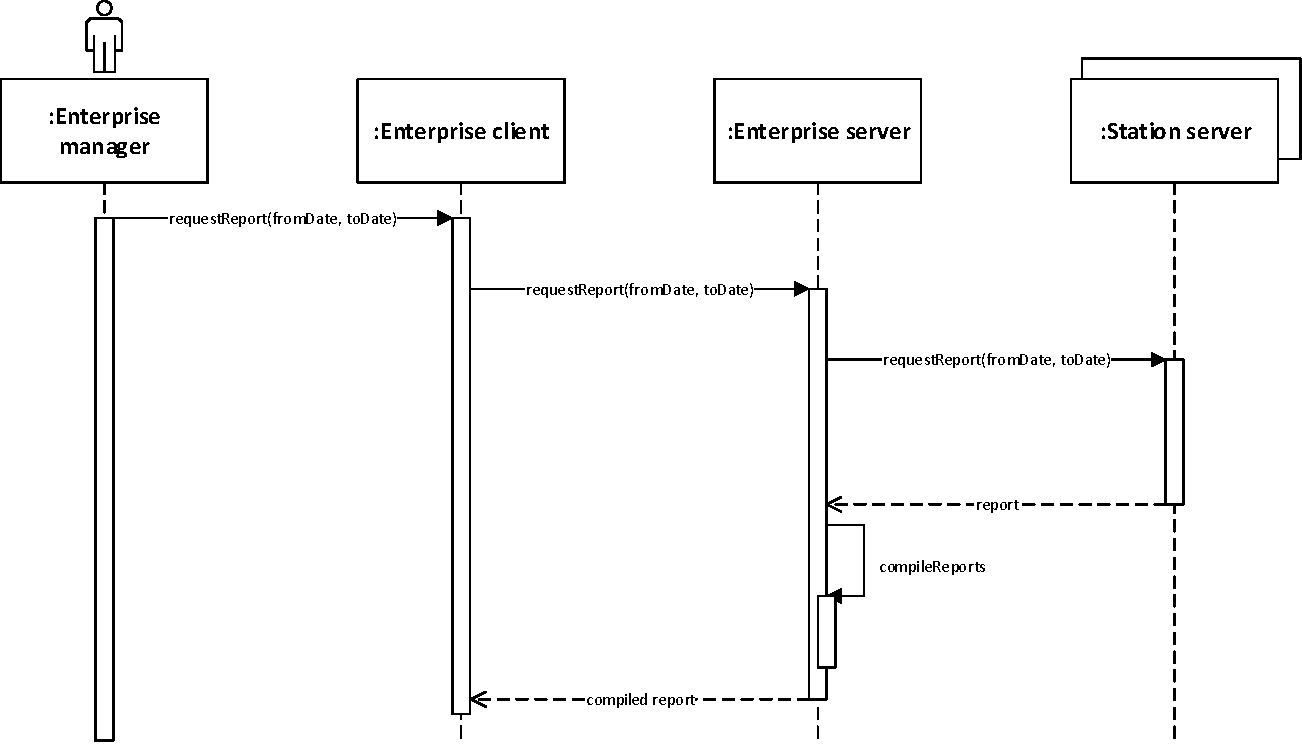
\includegraphics[width=1.4\columnwidth]{img/sequence_diagrams/sequence_diagram_show_reports}}
\caption{Sequence diagram of show report}
\label{fig:seq_show_report}
\end{figure}

\begin{enumerate}
\item The enterprise manager selects the time period he wishes to see statistics for.

\begin{enumerate}
\item The enterprise client user interface receives the call \texttt{requestReport} with the to and from date.
\item The enterprise client then sends the message \texttt{requestReport} to the enterprise server with the chosen date.
\item When the enterprise server receives the message from the enterprise client, it queries each station server with a \texttt{requestReport} with the specified dates.
\begin{enumerate}
\item When the enterprise server receives the first report from a station server, it starts to compile the final report using \texttt{compileReports}, taking in all new info as reports are received from the station servers.
\end{enumerate}
\item Once all reports are received and compiled, the compiled report is send back to the interface client.
\end{enumerate}
\item The system shows the full report with statistics from the selected time period.
\end{enumerate}
